% =====================================================================
%  Reduced 7-node WNT-APC-HOXA5/HOXA13-MYC-RA-CYP26A1 regulatory network
%  Schematic for the PINN inverse-problem study (colorectal-cancer WNT model).
%
%  Planar layout (no edge crossings). Directed edges (source -> target):
%    green arrow ->           = activation (+)
%    red bar-head -|          = inhibition (-)
%    blue dashed arrow ->     = external input / drive
%  APC sits at the centre so its three edges (to B, HOXA13, HOXA5) fan out;
%  the HOXA5 -| beta-catenin feedback is routed around the outside so the
%  whole drawing stays planar.
%
%  Compile with: pdflatex network_schematic.tex   (only needs tikz)
% =====================================================================
\documentclass[border=14pt]{standalone}
\usepackage{tikz}
\usetikzlibrary{arrows.meta, positioning, calc}

\begin{document}
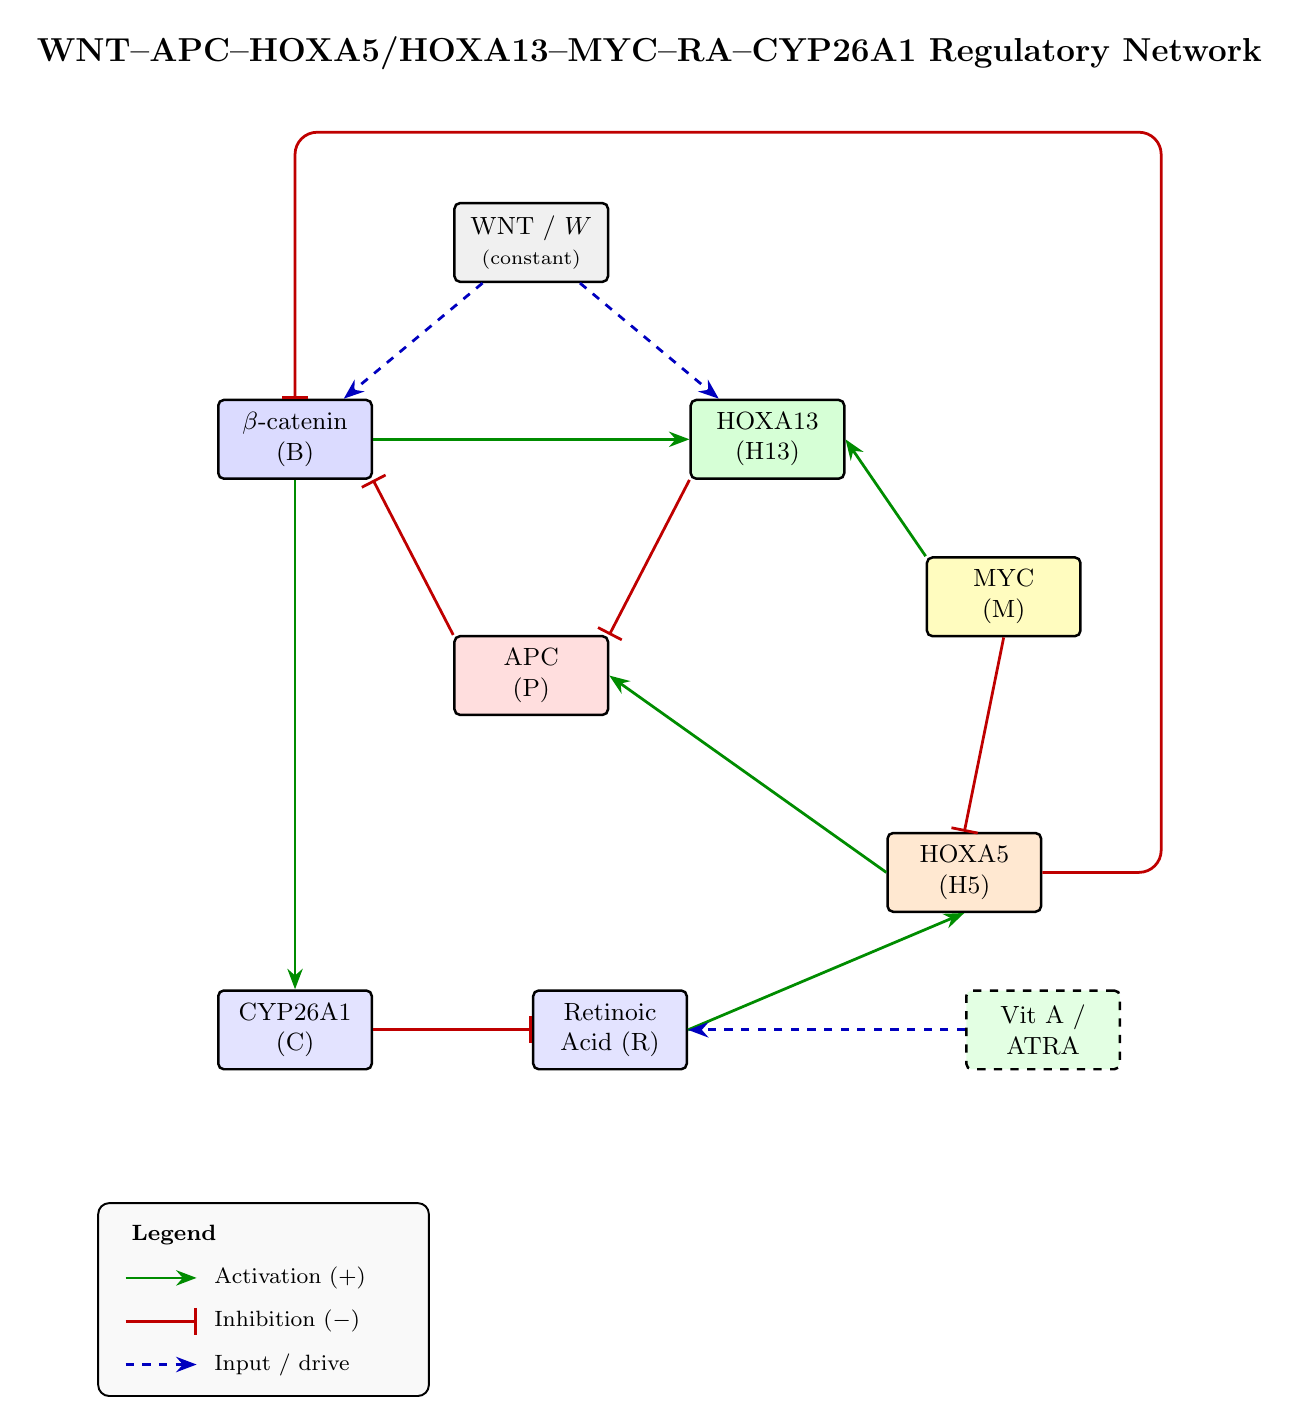
\begin{tikzpicture}[
  font=\small,
  rounded corners=2pt,
  nd/.style   ={draw, rounded corners=2pt, minimum width=1.95cm,
                minimum height=1.0cm, align=center, line width=0.9pt},
  % non-directional edge styles ------------------------------------
  act/.style    ={draw=green!55!black, line width=1pt, -{Stealth[length=2.6mm]}},
  inh/.style    ={draw=red!75!black,  line width=1pt, -{Bar[width=3.4mm]}},
  drive/.style  ={draw=blue!75!black, line width=1pt, dashed,
                  -{Stealth[length=2.6mm]}},
]

% =========================== TITLE ==================================
\node[font=\large\bfseries, align=center] at (6.5, 14.4)
  {WNT--APC--HOXA5/HOXA13--MYC--RA--CYP26A1 Regulatory Network};

% =========================== NODES ==================================
\node[nd, fill=gray!12]   (W)   at (5.0, 12.0) {WNT / $W$\\{\scriptsize(constant)}};
\node[nd, fill=blue!14]   (B)   at (2.0,  9.5) {$\beta$-catenin\\(B)};
\node[nd, fill=green!16]  (H13) at (8.0,  9.5) {HOXA13\\(H13)};
\node[nd, fill=red!13]    (P)   at (5.0,  6.5) {APC\\(P)};
\node[nd, fill=yellow!25] (M)   at (11.0, 7.5) {MYC\\(M)};
\node[nd, fill=orange!18] (H5)  at (10.5, 4.0) {HOXA5\\(H5)};
\node[nd, fill=blue!11]   (C)   at (2.0,  2.0) {CYP26A1\\(C)};
\node[nd, fill=blue!11]   (R)   at (6.0,  2.0) {Retinoic\\Acid (R)};
\node[nd, fill=green!11, dashed] (VA) at (11.5, 2.0) {Vit A /\\ATRA};

% ======================= ACTIVATION (green line) ====================
% beta-catenin -> HOXA13
\draw[act] (B.east) -- (H13.west);
% MYC -> HOXA13
\draw[act] (M.north west) -- (H13.east);
% RA -> HOXA5
\draw[act] (R.east) -- (H5.south);
% HOXA5 -> APC (numerator rho5*h5)
\draw[act] (H5.west) -- (P.east);
% beta-catenin -> CYP26A1 (straight down the left)
\draw[act] (B.south) -- (C.north);

% ======================= INHIBITION (red + bar) =====================
% APC -| beta-catenin (inhibition)
\draw[inh] (P.north west) -- (B.south east);
% HOXA13 -> APC
\draw[inh] (H13.south west) -- (P.north east);
% MYC -> HOXA5
\draw[inh] (M.south) -- (H5.north);
% CYP26A1 -> RA
\draw[inh] (C.east) -- (R.west);
% HOXA5 -| beta-catenin : feedback routed around the outside (top-right)
\draw[inh, rounded corners=8pt]
      (H5.east) -- (13.0,4.0) -- (13.0,13.4) -- (2.0,13.4) -- (B.north);

% ======================= DRIVES (dashed green) ======================
\draw[drive] (W) -- (B);
\draw[drive] (W) -- (H13);
\draw[drive] (VA.west) -- (R.east);

% =========================== LEGEND =================================
\begin{scope}[shift={(-0.2, -0.6)}]
  \draw[rounded corners, fill=gray!5, line width=0.7pt] (-0.3,0.4) rectangle (3.9,-2.05);
  \node[anchor=north west, font=\footnotesize\bfseries] at (0,0.25) {Legend};
  \draw[act]   (0.05,-0.55) -- (0.95,-0.55);
        \node[anchor=west, font=\footnotesize] at (1.05,-0.55) {Activation ($+$)};
  \draw[inh]   (0.05,-1.10) -- (0.95,-1.10);
        \node[anchor=west, font=\footnotesize] at (1.05,-1.10) {Inhibition ($-$)};
  \draw[drive] (0.05,-1.65) -- (0.95,-1.65);
        \node[anchor=west, font=\footnotesize] at (1.05,-1.65) {Input / drive};
\end{scope}

\end{tikzpicture}
\end{document}
